\chapter{Design} % (fold)
\label{cha:design}

    \section{Introduction}

    In this phase of the project the actual program has been designed according to the specification made earlier. Modules, classes, their relations, their attributes and their methods have been designed, a protocol for the communication between program instances has been established, and an interface has been designed. The work has been divided between the group members.

    This is a more technical description of the complex parts of our game. For a general description of our game, see the Specification Document.

    Our game will be called Bomb3D.

    % wat was onze policy wat betreft newpages ook weer?
    \newpage
    \section{Design decisions and assumptions}

    This section consists of an incomplete list of notable design decisions and assumptions, incomplete because we are probably unaware of certain decisions and assumptions. This is no problem as the list is not meant to be complete; creating it is merely a way of noting to our future selves that we have agreed on certain issues. For more design decisions, see the specification document, particularly the sections ``gameplay'', ``interface'' and ``winning the game''.

    \subsection{Design decisions}

    \begin{itemize}

        \item The game is played in ``tournaments'' that consist of multiple games, called ``games''. The total score over all games in the tournament determines a player's ranking in the tournament, with players getting one point for winning, none for losing (not winning).

    	\item Users can enter orders continuously. Programs act in turns, tens of times per second. When they act, they read their own player's input buffer queue, add it to the list of commands they got from peer programs, update the game's state according to this list, and send their player's input over the network to its peer programs. By the time their next turn comes around, each peer program will have sent its player's input to Bomb3D, so that it has a new list of commands to which to add its own player's commands.

        \item A level is rectangular and finite in size. There is a border around each level, that prevents a player from going beyond the level. Users can pick one of several different map files or make their own, to play in different levels.

        \item The assignment's intentionally vague food-gathering requirement will be incorporated into our program by the existence of ``power-ups'' in the level. Power-ups are an integral part of the game, that a player must utilise to gain the upper hand. A power-up appears whenever a ``soft block'' is destroyed, and confers a bonus to the player which walks over it first; either the player gets more bombs at his or her disposal, or these bombs become more powerful, or some special bonus is conferred. Which bonuses are available depends on the tournament's rules, as set by its creator.

        \item The winner of a game is the last player surviving. To avoid overly long matches, a tournament's creator can choose a maximum time the game will take, after this time has passed the game is decided by the number of power-ups each player has gathered over the course of the game. If that amount is also equal between multiple players, the game has multiple winners. This, `` Bomberman'', is the game as it works according to the standard ruleset, there is support for the creator of a tournament to change these rules.

        \item ``Bomberman'' is the ruleset we will focus on, though the tournament rules should allow for enough variation (for example: when does the game end?, how are points awarded?, which maps are used, which power-ups are available?, player stats?, players with different stats?) to allow for the playing of different kinds of games without fundamental changes.

        \item A consequence of the previous decision is that targeting and shooting should already be possible although it is not necessary for the ``Bomberman'' ruleset.

        \item ``Chaining'' is a problem we solved before designing the class diagrams. When a bomb explodes, it creates a blast radius. Everything in that radius; players, power-ups and soft blocks are destroyed. When a bomb belonging to a player is in that blast radius, that bomb also explodes. Chaining can be used strategically to make use of another player's bombs. We decided that whoever starts a chain ``owns'' the blast radius. Thus, when the bomb of player A explodes and chains with a bomb of player B, player A owns the blast radius. All players within the two blast radius' are killed and player A gets the score.

    \end{itemize}

    \subsection{Assumptions}

    Our assumptions are mainly of a technological nature: we are assuming that the network will be able to handle the traffic we are trying to get across it, and allow each program to act tens of times per second. We know from experience that this is probably a safe bet (given the amount of data that modern computer games manage to pass over the internet) as long as the data is efficiently encoded.

    We are not assuming anything about the operating system of the players. We will attempt to have Bomb3D work under Windows (XP), Mac OS X and Linux.
    

    \subsection{Reflection}
    Unfortunately we were not able to implement some of the design decisions. The game doesn't consist of a tournament with several games. In fact you only play one game. Also players cannot make their own levels that easy. Time was lacking to do so. All the other design decisions are correctly implemented.
    The network is able to handle all the traffic, but the speed is slow. We assumed that each program acts tens of times per second, but in practise the token went game 5 times per second. Because of this the multiplayer game is really slow. The rulesets as we designed weren't implemented, in favour of an event system on wich scripts can register.

    \section{Program modules} % (fold)
    \label{sec:program_modules}

      \subsection{The overall design} % (fold)
      \label{sub:design}
        The program consists of a framework running code from the following five modules, in four different threads:

        \begin{enumerate}
          \item The Input module. During a game, it gets input from the player through the mouse and keyboard and puts that input into a queue ($2$) from which the engine module will read.

          \item The network module

          \item The Output module. During a game gets input from the engine module through a queue, then shows the new situation to the player through, among others, the 3D graphics and the minimap. This module runs in the same thread as the Engine module.
          \item The Engine module. During a game, it gets input from the input module ($2$) and the multicast module ($1$) through two queues, updates the state of the game, puts the updated state data into a queue of the network module ($3$), and into a queue for the graphics/sounds module ($4$). It is the engine that handles the mathematical model of the tournament and everything needed for playing the game.
        \end{enumerate}

        The modules go together as shown in Figure~\ref{fig:modules}. In the next section, we will discuss how the separate modules are designed.\\

        \begin{figure}[!ht]
          \centering
          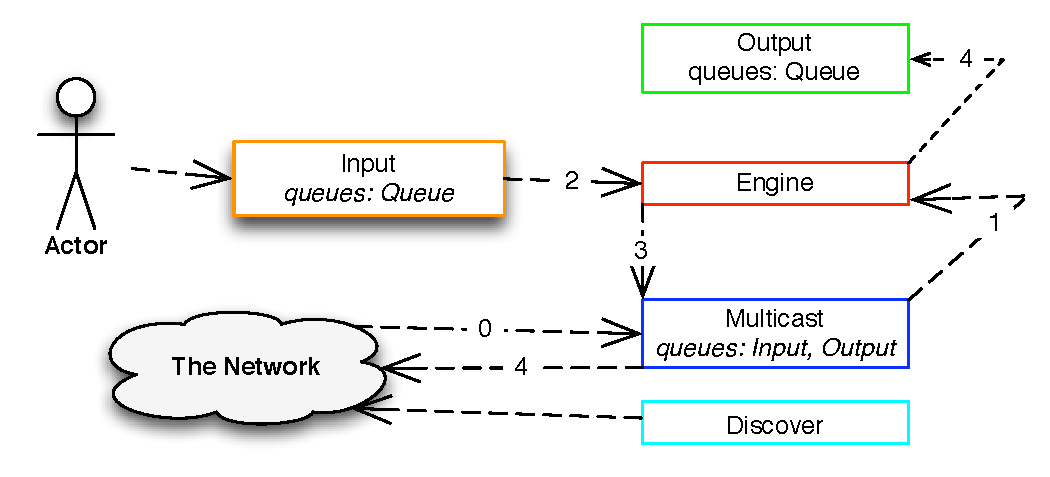
\includegraphics[width=11cm,height=5cm]{diagrams/modules}
          \caption{The 5 modules} \label{fig:modules}
        \end{figure}

        Our game runs in a cycle that is supposed to run many times per second. This means that we assume a certain network and processing speed to be available for playing this game; enough to update every player's screen dozens of times per second and sending and receiving network data. We do not believe that this is unrealistic, given the fact that many games manage to run in this way. We will, however, have to make design decisions which keep Bomb3D efficient.

      % subsection design (end)

      \newpage
      \subsection{UML Class diagrams}
      % TODO: Some more explanation.

        \subsubsection{The Input module} % (fold)
        \label{ssub:the_input_module}

          \begin{figure}[!ht]
            \centering
            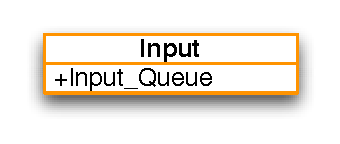
\includegraphics[width=4cm,height=2cm]{diagrams/UML_input}
            \caption{The class diagram for the Input module}
            \label{fig:UML_input}
          \end{figure}

          Figure~\ref{fig:UML_input} shows the input module. The input module handles all keyboard and mouse signals and puts these in the queue ``Input\_Queue''. The engine can access this queue and read all commands given by the player. PyGame will help us with reading player input, but during the writing of this section, we do not know how this should be implemented.
        % subsubsection the_input_module (end)

        \begin{figure}[!ht]
          \centering
          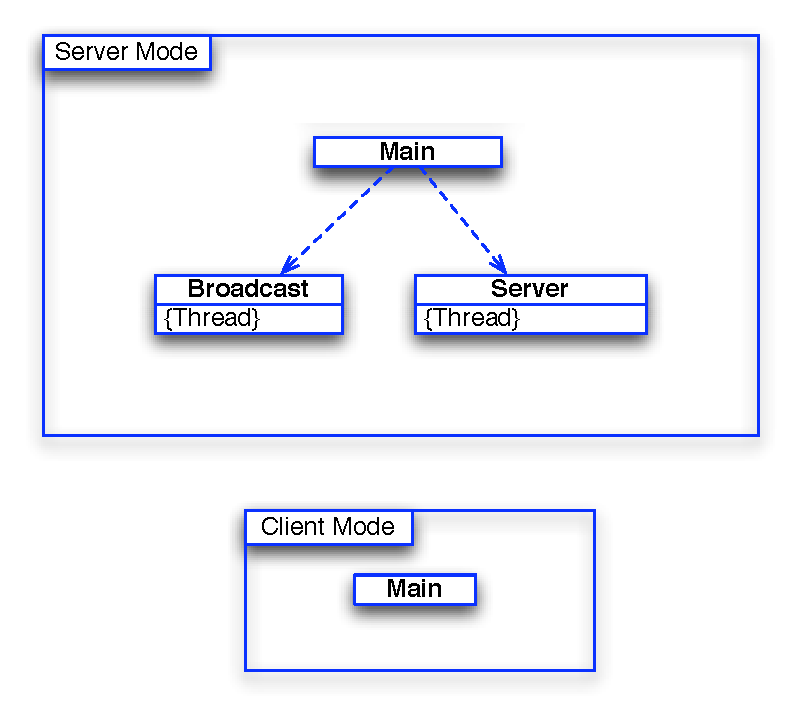
\includegraphics[width=6cm,height=8cm]{diagrams/UML_multicast}
          \caption{The class diagram for the network module} \label{fig:UML_multicast}
        \end{figure}

            \subsubsection{Starting the game and Discovery} % (fold)
            \label{ssub:starting_the_game_and_discovery}
                We use a client/server model for starting a game. One client creates a server, that sends a broadcast message to the entire network. All clients that are waiting to join a game, send a message back to the server. When the server times out, it tells every other client to whom he needs to connect. This makes a token-ring no longer requiring a server.
            % subsubsection starting_the_game_and_discovery (end)

           The blue Network class in Figure~\ref{fig:UML_multicast} is the same class in the network module diagram.

        % subsubsection the_discover_module (end)

        \subsubsection{The Engine module} % (fold)
        \label{ssub:the_engine_module}

          \begin{figure}[!ht]
            \centering
            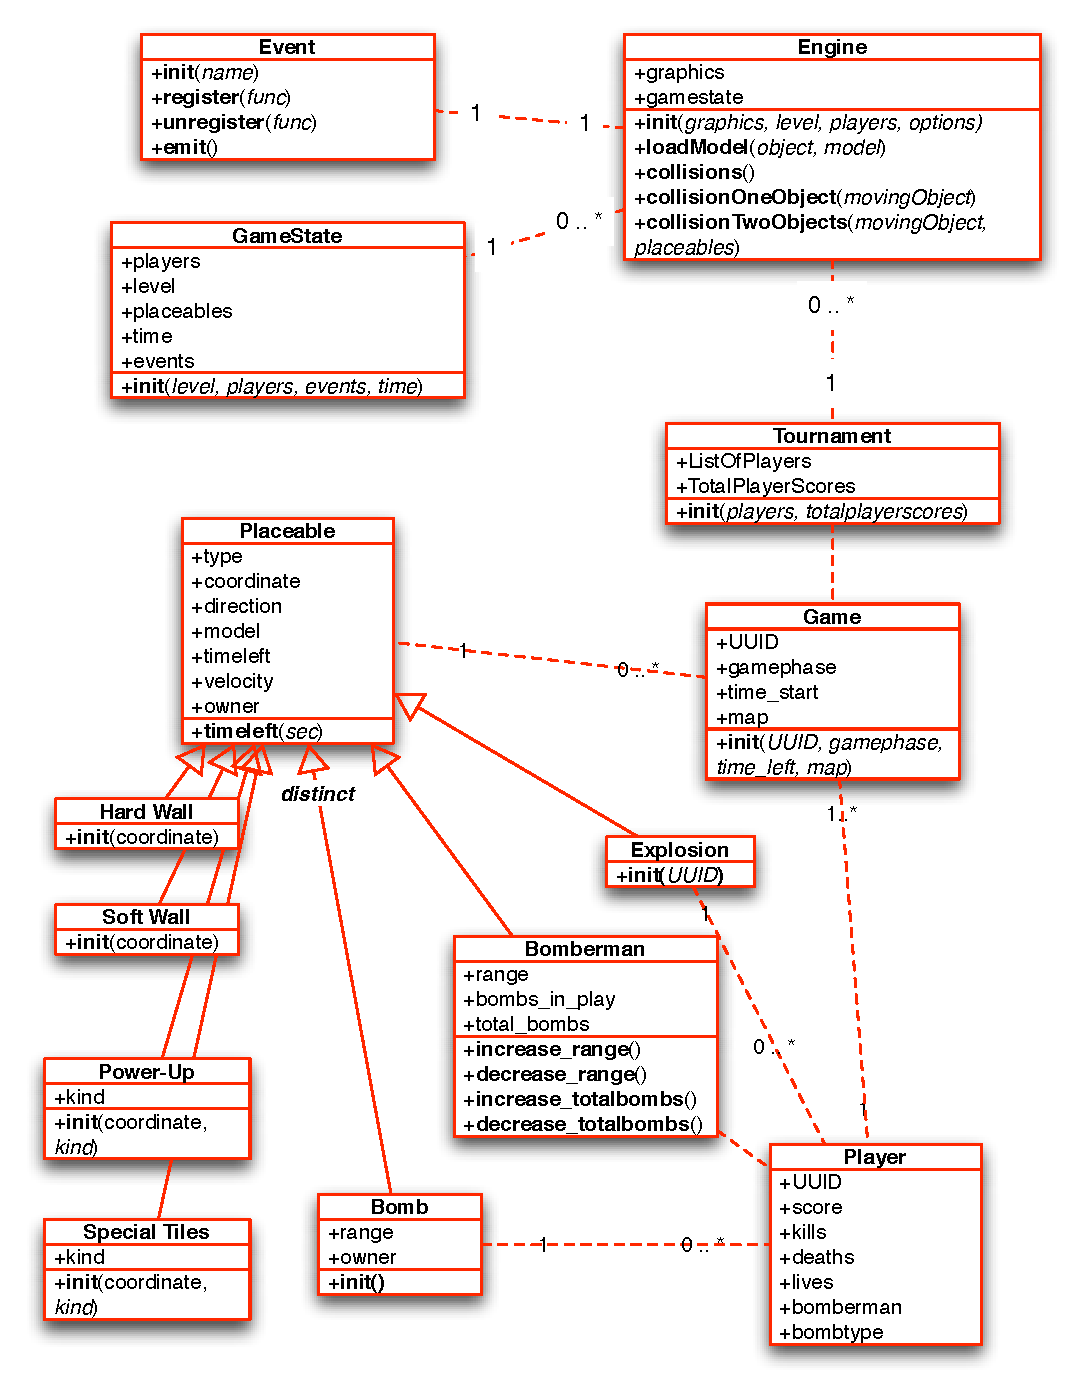
\includegraphics[width=12cm,height=14cm]{diagrams/UML_engine}
            \caption{The class diagram for the game Engine} \label{fig:UML_engine}
          \end{figure}

          \newpage

          A player starts playing the game by creating or joining a \emph{tournament}. A tournament consists of several \emph{games} or games that need to be won before an overall winner can be chosen. A game can have one or more players, though, of course, a game with one player in it is not very exciting. For every tournament there is a specific set of rules that states when someone wins or when anyone may join. The tournament class keeps track of all the different players and their total scores over the previous games in the tournament.

          Several games will be played in a tournament consecutively. Only 1 game may be active at any given time, that game will be ``InGame''. The game class handles ending the turn of a player and ending the game, making sure that all data goes to its right spot.

          Every game has its own data, like the time left to play the game. This data is in the \emph{Round} class.

          A \emph{Player} may only be busy with 1 game, he is either waiting to join or he is playing in the active game. This class keeps tracks of the player's score, how many times he has died, where it's standing and what bombs and upgrades belong to it. It also get's the input from both the input module and the multicast module. A player can place a request to move at the controller and to place a bomb.

          The \emph{Level} class keeps track of the size of the board and the lay-out.

          Several objects can be placed in a level. These objects share some properties, brought together in the \emph{Placeable} class. This consists mainly of a location (coordinates) and a texture. A placeable object is one of four types: Hard wall, Soft wall, Explosion or Bomb.\\
            \begin{enumerate}
              \item Hard Wall: this is an object that a player cannot interact with. Placing these wall creates a battle field through wich the player must maneuver, or use to his advantage when placing bombs.
              \item Soft wall: these are wall that can be destroyed by an explosion, but a player pass through it. This gives a player more objects to maneuver through, but can also be used to easily trap a player. When a soft wall is destroyed, it may ``drop'' a \emph{Power-Up} for the player or reveal a special tile.
              \item Bomb: a bomb belongs to a player and blows up when it's timer has reached zero. No player may walk through a bomb, not even it's owner. A player can use this ability to trap another player, but he can also accidentally trap himself.
              \item An explosion: When a bomb explodes, it create cross-shaped explosions, extending horizontally and vertically. These explosions have a place, a short duration of time and an owner. An explosion can set off other bombs, or destroy players, soft walls and power-ups.
            \end{enumerate}

          As has been said before, soft walls which are blown up can leave Power-Ups or reveal a special tile. Power-ups can be, but is not limited to, an increase of range, more bombs, different bombs, and a placeable soft wall \ldots

          A special tile could be a tile that propels a player forward, a tile that changes the direction of an explosion or a tile that transports a player. Special Tiles are not part of basic gameplay and will only be implemented later in the implementation proces.

      Initially, a level consists of coordinates that may have an associated object, like a wall block (indestructible) or a soft-block (destructible) or upgrade (destructible).

          As been said before, soft wall can drop Power-Ups or it can reveal a special tile. A Power-up could be, but not limited to, an increase of the range of your bombs, more bombs to be placed on the field, different bombs, a placeable soft wall \ldots

          A special tile could be a tile that propels a player forward, a tile that changes the direction of an explosion or a tile that transports a player. Special Tiles are not part of basic gameplay and will only be implemented later in the implementation proces.

    \subsubsection{Events} % (fold)
    \label{ssub:events}
        To connect the engine to the game logic, and to keep that connection flexible and extensible, we are going to use events.
        Events are things that can happen in a game, for example a player dies, a collision occurs, even a player who presses a key.

        Events often require something in the gamestate to change. For example when a player dies, he has to be removed from the game and points have to be given to the killing player. And when a player walks against a wall, a collision occurs and that player has to be stopped. So to do that, we'll introduce scripts that handle those things.

        A script is a piece of code that is interested in one of more events. So when that event happens, that piece of code gets called and makes changes to the gamestate accordingly.

        The big advantage of using events this way is that the engine stays very clean, and the game logic can easily be adjusted. We could easily make a shooter or a tetris game in this engine!
    % subsubsection events (end)

      % subsubsection the_game_module (end)

      \newpage
      \subsubsection{The Output module} % (fold)
      \label{ssub:the_output_module}

      \begin{figure}[!ht]
         \centering
         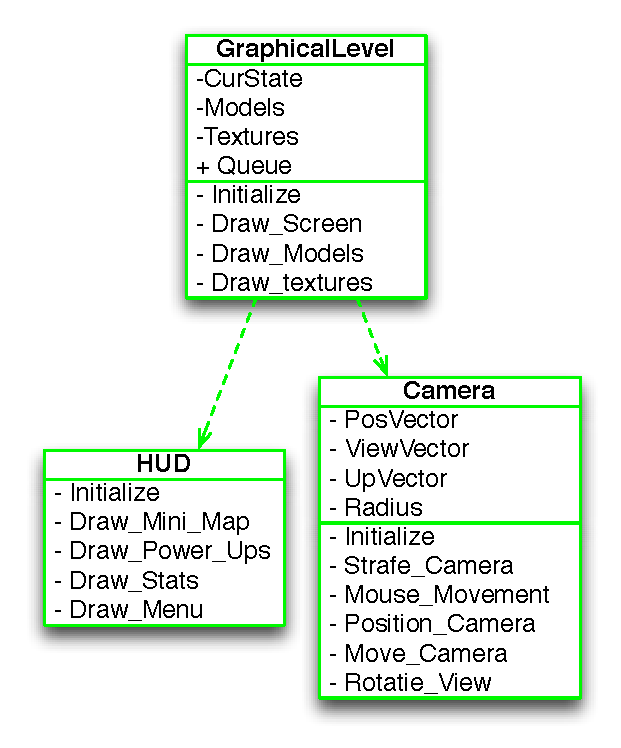
\includegraphics[width=8cm,height=10cm]{diagrams/UML_output}
         \caption{The class diagram for the game's Graphics}
         \label{fig:UML_output}
       \end{figure}

    \subsubsection{Screen} % (fold)
    \label{ssub:screen}
        The Output module gets a game state as input from the game engine and updates the screen. This screen consists of a 3D level and 2D layer on top of the 3D level. The 3D level is drawn according to the view of the camera and consists of a 3D world with all kinds of objects. The 2D layer consists of a minimap, the player's stats, and the player's power ups, which are all drawn. The Graphics module consists of three classes, namely: the GraphicalLevel class, the HUD class, and the Camera class.

           The GraphicalLevel class is the 3D level. It keeps the current game state, the models that are to be drawn and the textures that are used. After it is initialized, it can draw the 3D scene, draw the models, and apply the textures. The main use of this class is updating the 3D level based on the game state delivered by the game engine. It makes use of the two other classes to fully update the screen.

           The HUD class is a 2D layer on top of the 3D level. It draws the mini map, the power ups, the stats, and possible an in-game menu when activated. This class is used to update the 2D HUD layer on top of the 3D level based on the game state delivered by the game engine.

           The Camera class handles the camera movement. It can move the camera forward and backward, left and right, and rotate the camera, according to the player input delivered by the game engine. It is used as first-person view in the 3D level.
    % subsubsection screen (end)

    \subsubsection{Sound} % (fold)
    \label{ssub:sound}
        The Output module will also handle sounds when we have time left to implement it. There are some basic sounds stored, like explosions, walking etc. which will be played at certain in-game events. This means that certain keys and events will toggle a certain sound. For example when a player gets killed or kills, when a player has won, pressing an ``Activate powerup'' key etc.

           All the sounds will be implemented in the GraphicalLevel class, since the sounds ``change'' the 3D level. The sounds don't change the 3D level physically, but they do change the experience in the 3D level.
    % subsubsection sound (end)
       
         % subsubsection the_output_module (end)

    \subsection{Reflection}
    
    About the output module: We do not have 3D models for the objects displayed in the game; we use simple geometric shapes instead. This does not detract from the enjoyment of the game. In the HUD, the player cannot resize the minimap but otherwise things work smoothly. The sound also works.\\
\\
    About the engine module: The engine works, and customizing the scripts is not as easy as we imagined it could be. The engine code is stable, though it does not contain all features which we wanted to include, and so things which should have been customizable are hardcoded instead. The engine has been connected to the rest of the game relative late due to time pressure, so debugging it took a lot of time.\\
\\
    About the input module: this works fine.\\
\\
    About the network module: This works well as long as the player is in-game. The module has unfortunately turned out to be too simple in its design to have much use in the framework menus, which has caused us to drop many options (such as an easy way to choose a map and ruleset, and chatting before the game) which were originally planned. This module also cost us a lot of debug time.\\
\\
    Overall: Bomb3D works more or less as it should. There were some synchronisation issues during early testing, but as far as we know these are now resolved through standardisation of the framerate. Bomb3D does run too slow, though, which impedes proper testing. The modules communicate very well, there's no problems there.\\        
         
    % section program_modules (end)

    \section{Interpeer messages}
    \subsection{Introduction}
    For all peers to be on the same page, they need to communicate. And to understand each other, we need a protocol. That is what will be defined here.

    Messages will be encoded as a JSON object. We chose this because it is easy to read and write, for both humans and computers, it is compact and it can send complex datastructures. More information can be found on http://www.json.org.

    Every message has a sender property, to indicate who has send the message. Also, every message has a type, to indicate what kind of message it is. And depending on the type of message, there are some more arguments, which are described below.

    \textbf{Some examples}:

    To send the chat message ``Hello, world!'', this message should be transmitted:
    \begin{verbatim}
    {"sender"="UUIDOFSENDER", "type"="chat", "message"="Hello, world!"}
    \end{verbatim}

    To tell the other peers that you accepted the token, and to check the gamestate, this message should be transmitted:
    \begin{verbatim}
    {"sender"="UUIDOFSENDER", "type"="begin", "gamestate"="HASHOFTHEGAMESTATE"}
    \end{verbatim}

    To inform a new peer about the other peers, this message should be transmitted:
    \begin{verbatim}
    {"sender"="UUIDOFSENDER", "type"="networkstate",
        "peers"=[{"UUID"="UUID1","IP"="10.0.0.1"}, {"UUID"="UUID2","IP"="10.0.0.2"}]}
    \end{verbatim}

    \subsection{Messages}
    \begin{itemize}
      \item \textbf{Network related messages} \\
      These messages are necessary to get the network up and running, and to pass the token to everyone in the tokenring.
        \begin{itemize}
          \item \textbf{connect}
    A new peer sends this message to request to join the game. This message must not be forwarded.\\
    Arguments: \\
    \textit{version}: the version of the program you are running. \\

          \item \textbf{join}
    Used by the first peer to tell other already connected peers that a new peer has joined the network. This message can only be send if you control the token.\\
    Arguments: \\
    \textit{newPlayerUUID}: the UUID of the new player. \\
    \textit{newPlayerIP}: the IP of the new player. \\
    \textit{nickname}: the nickname of the new player. \\

          \item \textbf{networkstate}
    Communicates the current state of the network to a new peer. This message must not be forwarded.\\
    Arguments: \\
    \textit{peers}: an array of objects containing UUID and IP values of all peers in the netwerk. \\

          \item \textbf{begin}
    During a game, this communicates to the peers that you accepted the token, while passing a game state hash to check for possible desync faults (game state differences between peers).\\
    Arguments: \\
    \textit{gamestateHash}: a hash of the game state. \\

          \item \textbf{pass}
    During a game, this communicates that you pass the token on to another peer.\\
    Arguments: \\
    \textit{nextPlayerUUID}: the UUID of the next player. \\

          \item \textbf{part}
    This ends the game when a network problem has arisen (i.e. a disconnected peer).\\
    Arguments: None. \\

          \item \textbf{desync}
    This ends the game when a difference in gamestate is detected.\\
    Arguments: None. \\

        \end{itemize}

      \item \textbf{Initialization messages} \\
      These messages are to initialize the game and get everything started.
        \begin{itemize}
          \item \textbf{level}
    This tells the peers which level is being used in the current game, so that they can load the level file. This message can only be send if you control the token. \\
    Arguments: \\
    \textit{levelname}: the name of the level. While we don't have an option to send level files to other players, all players should have this level installed.\\

          \item \textbf{ruleset}
    This tells the peers what the ruleset is for this tournament. This message can only be send if you control the token.\\
    Arguments: \\
    \textit{ruleset}: an object containing key, value pairs containing the rules for the tournament (i.e. how many games should be played, a time limit, etc.). \\
        \end{itemize}

      \item \textbf{Game related messages} \\
      These messages are to communicate about what happens in the game.
        \begin{itemize}
          \item \textbf{input}
    This tells the other peers which input has been given. They need this input to update the game state and act accordingly. This message can only be send if you control the token.\\
    Arguments: \\
    \textit{key}: the key that was pressed. This is not the fisical key, but the logical action that that player has associated with that key. \\
    \textit{time}: the gametime the key was pressed. \\
    \textit{order}: the place of the input message in relation to other input messages sent at the same game time. \\

          \item \textbf{chat}
    This transmits a chat message to all peers. This may be send at any time. \\
    Arguments: \\
    \textit{message}: the chat message. \\

        \end{itemize}
    \end{itemize}

    \begin{figure}[!ht]
      \centering
      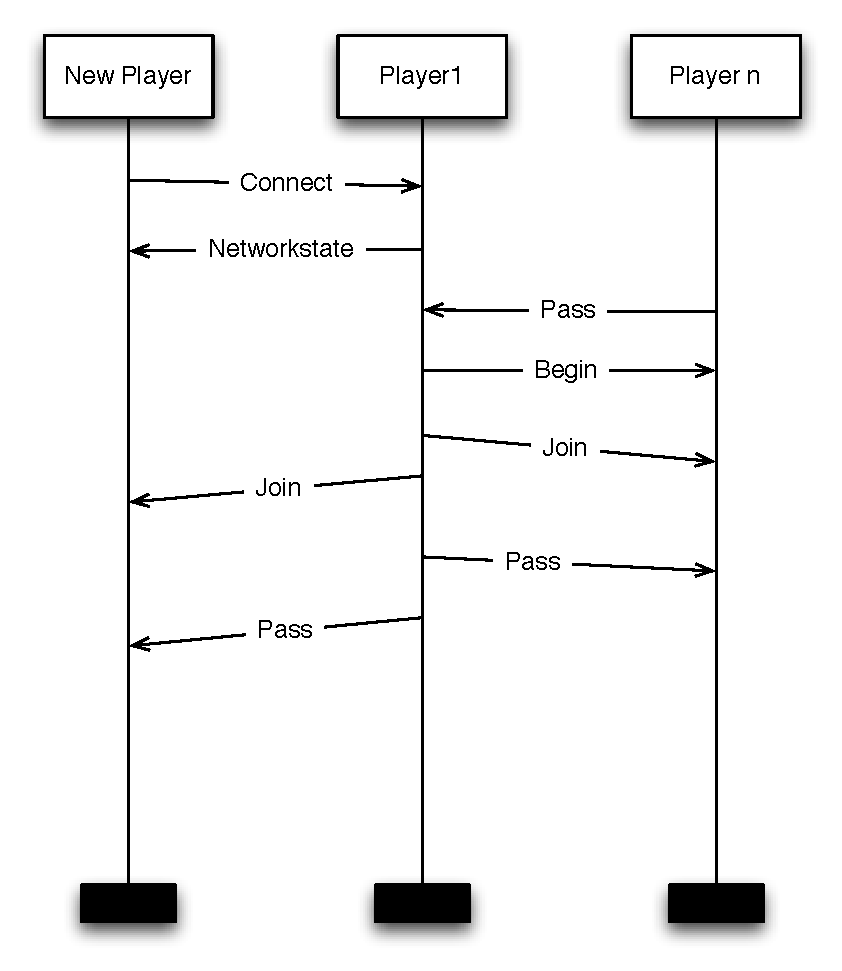
\includegraphics[width=0.5\textwidth]{diagrams/MSC_join}
      \caption{A player joins the game} \label{fig:MSC_join}

      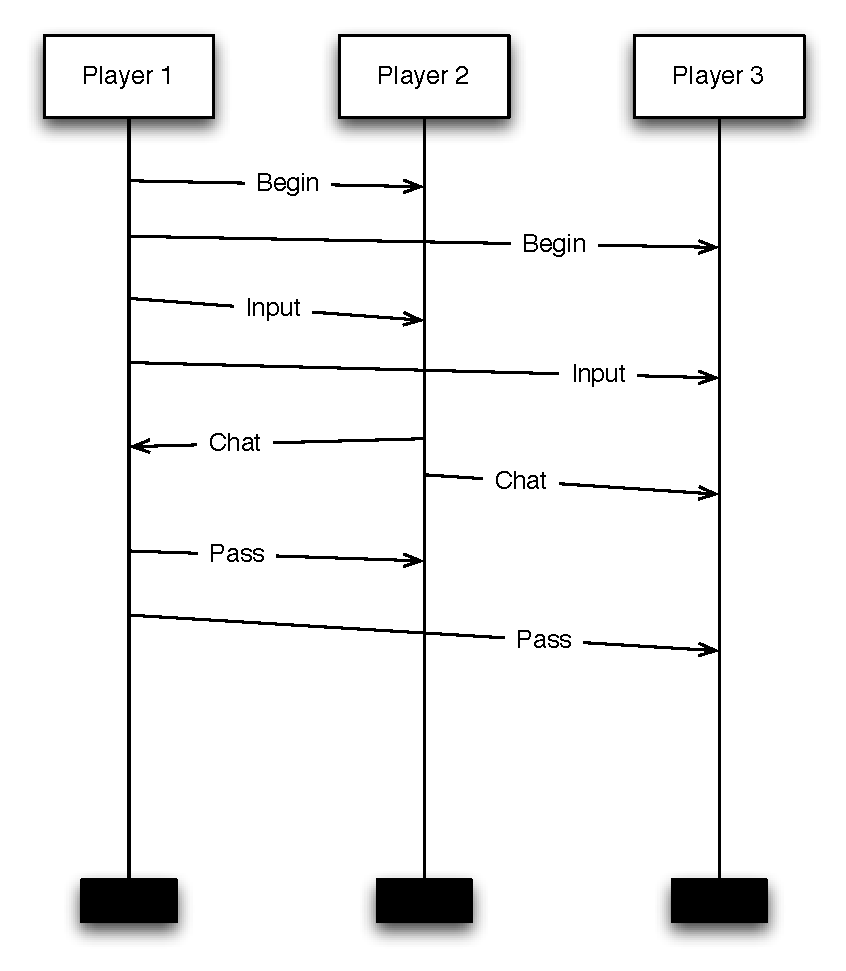
\includegraphics[width=0.5\textwidth]{diagrams/MSC_turn}
      \caption{A scenario during the game} \label{fig:MSC_turn}

      \caption{MSCs of 2 typical game situation} \label{fig:MSCs}
    \end{figure}


    \subsection{Extension options}
    We thought of some options to extend the protocol. They are needed for options that are low on our priority list, so we will not design them right now, we will just give a short description.

    \begin{itemize}
     \item Join a running tournament \\
     To make it possible to join a tournament that is already running, some information on the current tournament should be transmitted.
     \item Recover from a network error (i.e. a disconnect from a player) \\
     When a player disconnects, the other players have to make a new network, without loops and preferably without losing more other players, so some extra communication should be introduced to make that possible.
     \item Level transfer \\
     If we have support for multiple maps, it could happen that some of the players don't have the map that is going to be played. In that case it would be nice if the map will be send to that player.
    \end{itemize}

    \subsection{Reflection}
    The interpeer messages work as they are described here. There are no problems with the messages, and the network works fine. Only the the token goes game five times per second, which is really slow. We don't know what exactly causes the token to travel at such a low rate. The extension options are not implemented simply because we didn't have time to do so, and there were other priorities during the implementation phase.

    \newpage

    \newpage
    \section{Division of work}

    \begin{itemize}

      \item Output: Leroy, Edin, Neal

      \item Network, Input: Jeroen, Anson

      \item Framework, Engine: Stef, Etienne, Edin

      \item Final document, Manual: Anson

      \item Menus: Anyone with spare time.

    \end{itemize}

    The output and the engine will probably take most of the work, so both get two dedicated developers. These are Leroy and Neal for the output, because they have already done some exploratory work on the topic, and Stef and Etienne for the engine, for the same reason.

    Building the networking and input modules will yet take some time, but it is not as much work as building the above two modules, so it will get just one dedicated developer. This will be Jeroen, who has already designed the network's overall structure.

    Anson will work mostly on documentation, because he has already coordinated the documentation earlier in the project. He will also assist the network module's developer, particularly during the early stages, when assistance will be very helpful.

    Edin will help the engine developers early on, when the design of the framework will take a lot of their time. He will move on to assisting the output developers later in the project, when they will have more work. This will have the added benefit that the output developers will have someone working with them who has some knowledge of the engine.

    The menus will be created by anyone with spare time. They can be made as simple or as elaborate as we want, and their looks are not essential to the gameplay, so the amount of time spent on them can be more or less as large or as small as we see fit.
    
    \subsection{Reflection}
    The division of work as written above, actually worked pretty well. Everyone had there own tasks and everyone could work independently when needed. Also most of the group worked on different tasks than they were scheduled when this was needed. This was the case at the end of the project when everyone has fixing bugs and typing the documentation. Although the game didn't turn out exactly the way we wanted, we think that the division of work wasn't the problem.

% chapter design (end) 
